\section{Chameleon Framework}
\label{sec:PoC-Chameleon}
\index{PoC!Chameleon}

Chameleon is implemented in C++ based on hybrid MPI+OpenMP. In an MPI process, we can deploy multiple OpenMP threads for executing tasks and a dedicated thread (called $Tcomm$) for overlapping communication \& computation. $Tcomm$ is deployed using POSIX thread (\texttt{pthread}). Task-based parallel applications with Chameleon can run efficiently on shared and distributed memory systems. We mainly use $Tcomm$ to deploy our proactive load balancing approach, where our implementation can be called a proactive load balancing tool (or proactive LB tool for short).\\

%The mechanism and design of this implementation are described as follows:
%\begin{itemize}
%	\item First, the Chameleon framework is introduced in Subsection \ref{subsec:chameleon}.
%	\item Second, we present the design and how our balancing tool is integrated with Chameleon.
%	\item Finally, we show an example of how they are put together in practice.
%\end{itemize}

Note that in Chameleon itself, this framework already provides the reactive load balancing approach. As explained in Chapter \ref{ch:wstoreactlb}, Section \ref{sec:relatedwork}, reactive load balancing follows a push-oriented mechanism, where tasks are offloaded from overloaded to underloaded processes. In other words, we can say that tasks are offloaded from a slow to a fast process. This is different from a pull-oriented mechanism in work stealing.\\

The Chameleon framework is described through its task system and how tasks are managed, as the following subsections:
\begin{enumerate}
	\item Migratable task definition: explains the structure of tasks defined by task properties and relevant methods in terms of implementation. For task migration at runtime, tasks must be migratable. Therefore, this subsection will show the definition of a migratable task in Chameleon.
	\item Task execution and communication thread: explains the structure and implementation of the task manager in Chameleon. This implies the mechanism by which tasks are scheduled and mapped to resources for execution. Importantly, this subsection introduces an overview of the dedicated thread for communication and task migration. 
\end{enumerate}

%\noindent \textbf{A. Migratable task definition}\\

\subsection{Migratable task definition}
\label{subsec:migratable_task}

\begin{figure}[t]
	\centering
	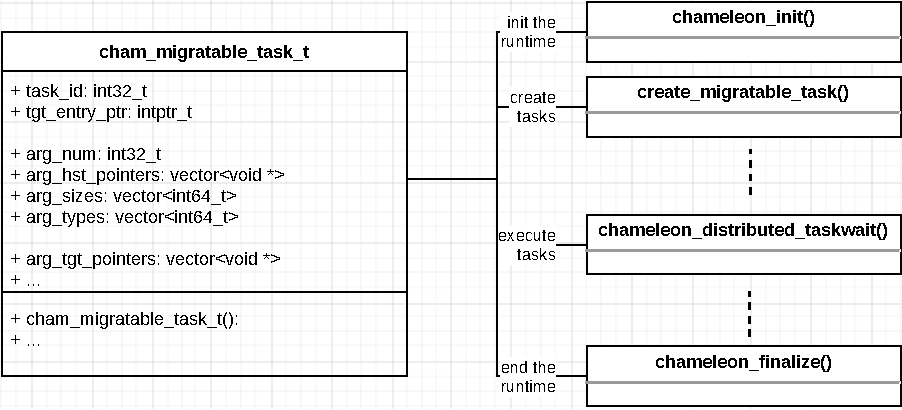
\includegraphics[scale=0.725]{./pictures/poc_implementation/poc_chameleon_class_and_comm_diagram.pdf}
	\caption{A combined communication diagram between the task class and main APIs of the Chameleon runtime.}
	\label{fig:poc_chameleon_class_comm_diagram}
\end{figure}

The implementation of Chameleon is a custom \texttt{libomptarget} plugin in LLVM OpenMP runtime \cite{llvm2013omp}. Hence, Chameleon enables declaring a task using directives, such as \texttt{\#pragma omp target}. For the data environment of tasks, we can use the clause \texttt{map} to specify. When a task is created, the compiler will manage appropriate calls, referring to the task entry function (code) and its data environment (data). Properties in implementation represent the code and data in a task.\\

Figure \ref{fig:poc_chameleon_class_comm_diagram} shows a definition of class \texttt{cham\_migratable\_task\_t} associated with the task properties, defining a task in Chameleon. This class is shown on the left side, detailing some essential attributes and a constructor function (named \texttt{cham\_migratable\_task\_t()}). On the right side, we illustrate the link between the initialization of a task and the main API functions in Chameleon.\\

Each task has a unique ID (\texttt{task\_id}, type \texttt{int32\_t}). When a task is migrated to another process, its ID stays the same for simply distinguishing between local and remote tasks. The following are some other important properties:
\begin{itemize}
	\item \texttt{arg\_num}: indicates the number of input arguments belonging to a task.
	\item \texttt{arg\_hst\_pointers}: indicates a vector of pointers that refers to the arguments of a task. Following this, there are related properties, such as argument sizes (\texttt{arg\_sizes}), argument types (\texttt{arg\_types}).
	\item \texttt{arg\_tgt\_pointers}: points to the remote side or remote process where a task will be executed if it is migrated.
\end{itemize}

When a task is offloaded onto a remote side, the same hybrid binary of the task is executed. Besides that, we address each task by an offset from the start of the loaded library to the corresponding task entry function. It is used to determine the correct entry point on a remote MPI process.\\

The class \texttt{cham\_migratable\_task\_t} allows us to pack and migrate tasks from one process to another. In practice, tasks can be generated by \texttt{create\_migratable\_task()}. The working flow of a task-based application written by Chameleon follows the main API functions shown in Figure \ref{fig:poc_chameleon_class_comm_diagram}, including:
\begin{itemize}
	\item \texttt{chameleon\_init()}: initializes Chameleon.
	\item \texttt{create\_migratable\_task()}: creates migratable tasks. Users specify tasks and the number of tasks.
	\item \texttt{chameleon\_distributed\_taskwait()}: distributes and executes tasks. The scale of computing resources, such as the number of compute nodes, processes, and threads per process, is configured by users.
	\item \texttt{chameleon\_finalize()}: finalizes the execution by Chameleon.
\end{itemize}

Behind these functions, tasks are managed to run in parallel (even on shared or distributed memory systems). From the side of users, we can consider applications as black boxes. Chameleon takes control of task execution. After that, the application flow is given back to users. The next subsection will explain the execution of tasks in Chameleon.

% task execution, communication thread, and reactive load balancing
%\begin{shaded}
%	\noindent \textbf{Task execution, communication thread, and reactive load balancing}
%\end{shaded}

%\noindent \textbf{B. Task execution, communication thread, and reactive load balancing}\\

\subsection{Task execution and communication thread}
\label{subsec:task-exe-Tcomm}

Like other task-based programming models, task execution in Chameleon is hierarchical. After tasks are created and distributed across processes, each will manage the execution of assigned tasks through its threads. Chameleon distinguishes OpenMP threads for executing tasks (called execution threads or worker threads) and a dedicated POSIX thread for communication between processes (named $Tcomm$). When imbalance occurs at runtime, the dedicated thread can migrate tasks to balance the load.\\

To ensure the execution of all local and remote tasks are synchronized, Chameleon requires a global synchronization barrier. Therefore, all communication between processes has to reach the synchronization barrier. In a process, all execution threads are triggered when \texttt{chameleon\_distributed\_taskwait()} is invoked. The dedicated thread is triggered when reactive load balancing is enabled. After tasks are assigned to each process, they are queued before scheduling to execution. There are two types of task queues: one queue of local tasks and one queue of remote tasks. The framework prioritizes the execution of remote tasks before working on local tasks because the original process might request the remote side to send back the results of their tasks.

Regarding the progress of execution threads and $Tcomm$, they are desbribed as follows:
\begin{itemize}
	\item The execution threads are created by OpenMP runtime, while $Tcomm$ is created by a POSIX thread ($pthread$). When $Tcomm$ is enabled, it monitors load status and exchanges the status continuously. The load status accounts for execution speed. In particular, Chameleon uses the queue length that indicats the number of remaining tasks. This determines which process is slow, which is fast, and imbalance ratio to make decisions for reactive load balancing.
	\item When an imbalance is detected, the operations performed on $Tcomm$ include:
		\begin{itemize}
			\item Select a victim to migrate tasks (offload tasks).
			\item Decide the number of tasks for migrating at once, where this number can be safely set one task at a time, or users can adjust it.
			\item Enable to receive back the results of migrated tasks.
			\item Stop or cancel all communication progress when the execution of tasks reaches synchronization barriers.
		\end{itemize}
\end{itemize}

\begin{figure}[t]
	\centering
	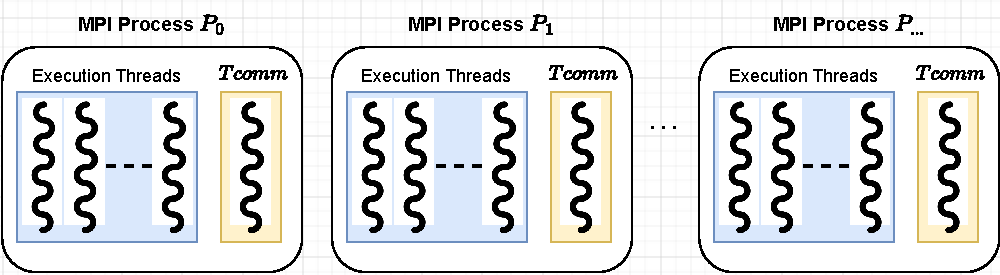
\includegraphics[scale=0.7]{./pictures/poc_implementation/poc_chameleon_and_commthread.pdf}
	\caption{Chameleon runtime with the dedicated thread for overlapping communication and computation.}
	\label{fig:poc_chameleon_commthread}
\end{figure}

Figure \ref{fig:poc_chameleon_commthread} illustrates the overview of processes and threads created in Chameleon. Horizontally, suppose we launch $P$ processes indexed from $0$ to $P-1$. One process is mapped to one CPU socket, where a CPU has multiple cores. The execution threads in a process are pinned to these cores, where the last core is off for running the dedicated thread $Tcomm$. In Figure \ref{fig:poc_chameleon_commthread}, we highlight execution threads with blue background, while $Tcomm$ with yellow background. A compute node in HPC clusters today often has two CPU sockets. Hence, to facilitate the execution of Chameleon with full cores, we can deploy two processes per node, and all threads map to all cores per a CPU socket.\\

For our proactive load balancing scheme, we can exploit $Tcomm$ to perform task characterization and load prediction, instead of only monitoring load. After training a prediction model, $Tcomm$ provides prediction knowledge about load values and distributes the values. Benefiting from predicted load values, we estimate which process is a potential victim and how many tasks should be migrated at a time. The implementation of our approach is designed as a plugin tool (refers to a callback tool like the OpenMP Tool interface \cite{eichenberger2013omptool}). $Tcomm$ will manage callback functions declared in the tool, allowing users to predefine events and functions needed for proactive load balancing. The next subsection shows our implementation as a Chameleon plugin tool.

% During execution, $Tcomm$ enables monitoring load, exchanging information, and offloading tasks.

\section{Proactive Load Balancing as a Plugin Tool} \label{sec:cham_proactlb_tool}

Users can interfere with the Chameleon operations via callback events that are designed similarly to the OpenMP Tool interface (OMPT)\cite{eichenberger2013omptool} \cite{supinski2022omptechreport}. Note that the term ``tool'' here indicates a callback tool used to interfere with the primary operations in Chameleon. Users can define the tool, so we sometimes call it as a plugin or user-defined tool. The idea is to implement the tool outside the main library to support different purposes, such as profiling tasks, load prediction, and load balancing algorithms. Therefore, we can create different tools. \\

Chameleon is developed with callback signatures and specific data types to define callback functions and their parameters in the tool. For the returned values of the callback functions, we can yield them to input the API functions in Chameleon. The tool can be initialized by linking and loading directly into Chameleon. \\

Figure \ref{fig:poc_chamtool_flowchart} shows a flowchart to explain how a callback tool is loaded and executed alongside the Chameleon framework. This flowchart refers to the OpenMP Tool scheme, where the Chameleon runtime is similar to the OpenMP runtime. During execution, the Chameleon runtime will examine the \texttt{tool-var} ICV\footnote{Internal control variables (ICVs) that control the behavior of the runtime. ICV stores information such as the address of the compiled tool externally.} as one of the first initialization steps. If the \texttt{tool-var} value is \texttt{null} or \texttt{disabled}, Chameleon will continue without checking the tool's presence, and the tool interface will be disabled (so-called \texttt{inactive}). Otherwise, if the tool interface is \texttt{active}, then change to \texttt{Pending} and \texttt{Find next tool}. If Chameleon finds the tool, it calls \texttt{cham\_start\_tool}. At this stage, there are two options to define \texttt{cham\_start\_tool}:
\begin{itemize}
	\item By statically linking the definition of \texttt{cham\_start\_tool} into Chameleon.
	\item By introducing a dynamic-linked library that includes the definitions of \texttt{cham\_start\_tool} into the application's address space.
\end{itemize}

We apply the second option with the illustration shown in Figure \ref{fig:poc_chamtool_flowchart}. Our definition of the tool is separate and shown as the interruptable region. The region shows \texttt{tool.h} and \texttt{tool.cpp}, where we define a data structure for profiled-tasks information (\texttt{prof\_task\_info\_t}). With \texttt{prof\_task\_info\_t}, we highlight some major properties such as \texttt{ttid} (task ID for tracking tasks at the tool side), \texttt{num\_args} (the number of input arguments in a task), and other time parameters like \texttt{que\_time} (when a task is queued), \texttt{sta\_time} (when a task is scheduled to execute), \texttt{end\_time} (when a task is finished), \texttt{mig\_time} (when a task is migrated to another process), \texttt{exe\_time} (task execution time which can be calculated by \texttt{sta\_time} and \texttt{end\_time}), \texttt{core\_freq} (the profiled information about core frequency where a task is assigned). The frequency can be measured directly before a task is executed. Explicitly, we present some primary methods in the tool that are invoked to characterizing tasks, training and loading prediction models. For example,
\begin{itemize}
	\item \texttt{on\_cham\_callback\_task\_create()}: is called after tasks are created. Thus, the tasks' features, including arguments and input data sizes, can be characterized.
	\item \texttt{on\_cham\_callback\_get\_task\_wallclock\_time()}: is called after tasks are finished. We can record \texttt{end\_time} and calculate \texttt{exe\_time}.
	\item \texttt{on\_cham\_callback\_train\_prediction\_model()}: is called to define a prediction model with input and output layers. The model is trained to predict the load values based on what we hint to characterize. In iterative applications, this callback can be triggered after several finished iterations. For example, we can configure a certain number of iterations before execution, such as 5, 10 iterations, to collect data and train a prediction model.
	\item \texttt{on\_cham\_callback\_load\_prediction\_model()}: is called to load a trained model. This callback is triggered after the return of \texttt{on\_cham\_callback\_train\_prediction\_model()} is available.
	\item Additional callback functions can be defined and added by users.
\end{itemize}

\begin{figure}[t]
	\centering
	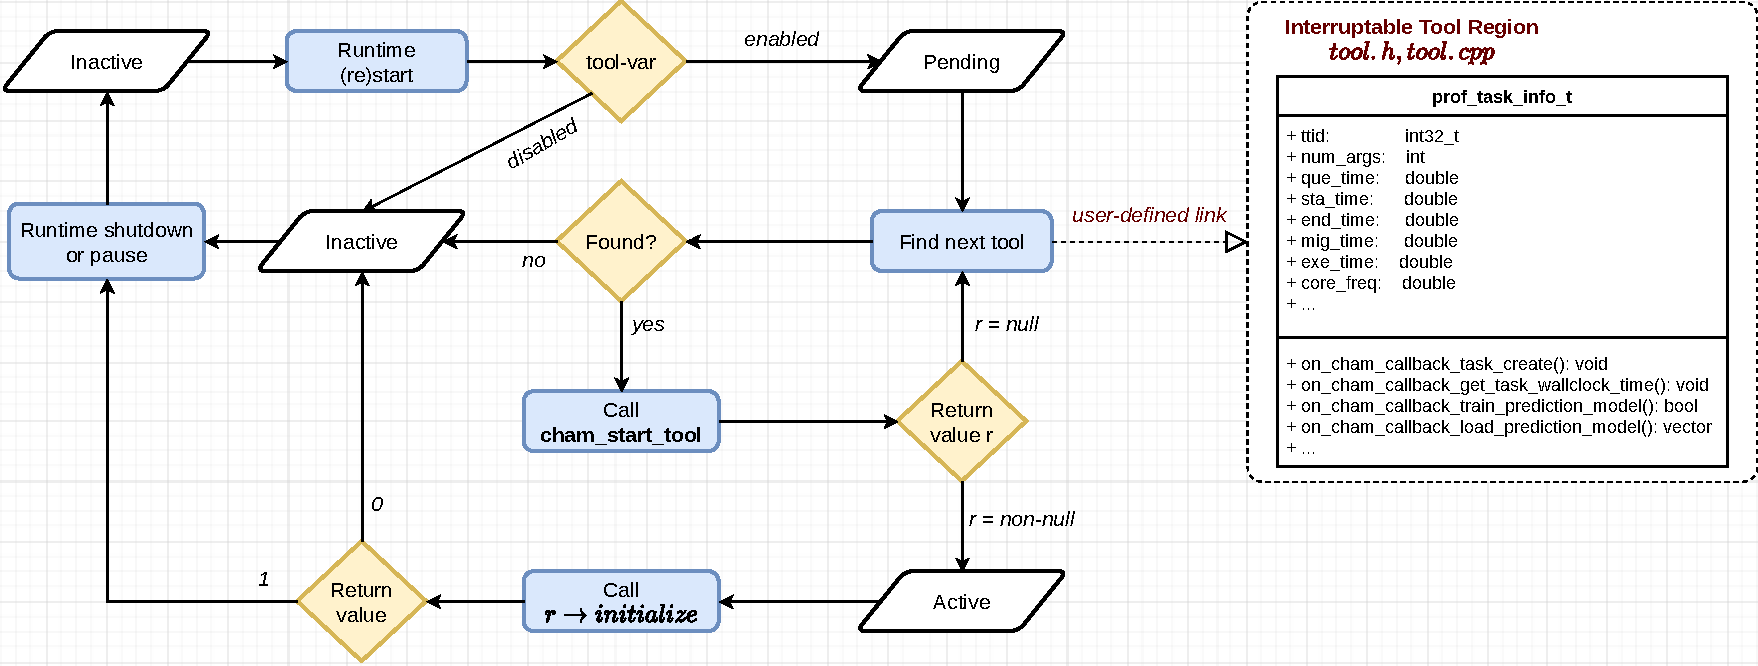
\includegraphics[scale=0.525]{./pictures/poc_implementation/poc_chamtool_flowchart.pdf}
	\caption{A flowchart and class linking to show how a plugin tool is loaded.}
	\label{fig:poc_chamtool_flowchart}
\end{figure}

In the case without online training, a pre-trained model for predicting load can be trained from the historical data. Then, we load it directly by the tool. The mechanism of this callback tool is intended to be flexible for developing different load balancing methods.

\section{Task-based Parallel Application as a Black Box} \label{sec:cham_proactlb_example}

As an example, we also use the synthetic \texttt{MxM} matrix multiplication to explain how the plugin tool and Chameleon work together. \texttt{MxM} is reproducible to conduct different imbalance scenarios. The tasks are defined by \texttt{MxM} compute kernels, indicating the function of calculating dense matrix multiplication $C = A \times B$. The input arguments include matrix $A$ and matrix $B$, while the output is matrix $C$, where their sizes reflect the wallclock execution time of tasks. We reveal a snippet code of \texttt{MxM} to introduce writing a task-based application with Chameleon \cite{Klinkenberg2020ChameleonReactLB}.

\begin{lstlisting}[language=C++, caption={A snippet code for implementing \texttt{MxM} compute tasks in Chameleon}, label={lst:cham_mxm_code}]
// MxM compute kernel defined as task
void mxm_kernel(double *A, double *, double *C, int mat_size);	
	
// Main function
inf main(int argc, char *argv[])
{
	// Chameleon, MPI initialization and matrix allocation, ...
	int N = matrix_size;

	// define tasks
	#pragma omp parallel
	{
		#pragma omp for nowait
		for (int i = 0; i < num_tasks; i++){
			double *A = matrices_a[i];
			double *B = matrices_b[i];
			double *C = matrices_c[i];
			
			#if USE_OPENMP_TARGET_CONSTRUCT // OpenMP target approach
				# pragma omp target map(tofrom: C[0: N*N]) map(to: A[0: N*N], B[0: N*N])
				mxm_kernel(A, B, C, N);

			#else // Chameleon API approach
				map_data_entry_t *args = new map_data_entry_t[4];
				args[0] = chameleon_map_data_entry_create(A,
												N*N*sizeof(double),
												MAPTYPE_INPUT);
				args[1] = chameleon_map_data_entry_create(B,
												N*N*sizeof(double),
												MAPTYPE_INPUT);
				args[2] = chameleon_map_data_entry_create(C,
												N*N*sizeof(double),
												MAPTYPE_OUTPUT);
				args[3] = chameleon_map_data_entry_create(lit_size,
												sizeof(void *),
												MAPTYPE_INPUT|MAPTYPE_LITERAL);
				cham_migratable_task_t * cur_task =
												chameleon_create_task((void *)& mxm_kernel, 4, args);
				chameleon_add_task(cur_task);
			#endif
		}
		
	// trigger task execution and reactive load balancing in the background
	chameleon_distributed_taskwait();
	}

	// Chameleon, MPI finalization and clean up ...
	...
}
\end{lstlisting}
\hfill

\begin{figure}[b]
	\centering
	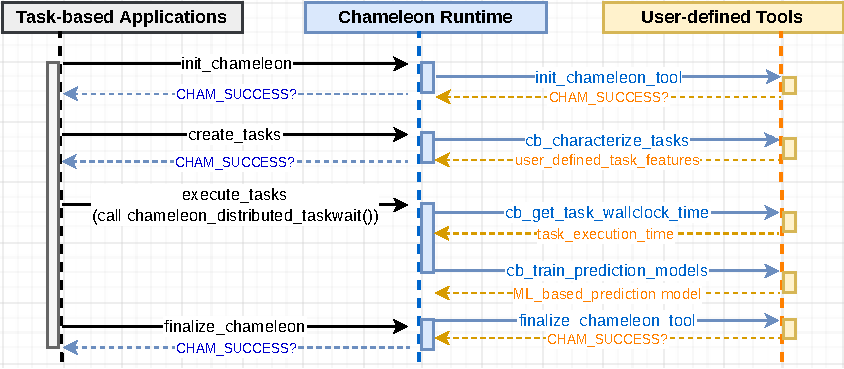
\includegraphics[scale=0.7]{./pictures/poc_implementation/poc_sequence_diagram_chamtool.pdf}
	\caption{A sequence diagram of runtime behaviors between applications, Chameleon, and tool.}
	\label{fig:poc_chamtool_sequence_diagram}
\end{figure}

Listing \ref{lst:cham_mxm_code} shows a snippet code example of defining \texttt{MxM} compute tasks. The task code entry points to the function \texttt{mxm\_kernel()}, where the inputs of a task include four arguments, i.e., matrix $A$, $B$, $C$, and \texttt{lit\_size}. Argument \texttt{lit\_size} implies the literal size of matrices. Following here, tasks are generated by the function \texttt{chameleon\_create\_task()} and queued by \texttt{chameleon\_add\_task()}. To execute tasks, we call \texttt{chameleon\_distributed\_taskwait()}. This function implicitly performs task execution in parallel.\\

Figure \ref{fig:poc_chamtool_sequence_diagram} presents the interaction workflow between the application, Chameleon, and tool. The workflow has three columns: Task-based Applications, Chameleon Runtime, and User-defined Tools. Corresponding to the snippet code of \texttt{MxM}, the side of application starts with initializing Chameleon (shown as arrow \texttt{init\_chameleon}), then creating tasks (arrow \texttt{create\_tasks}), executing them (arrow \texttt{execute\_tasks}), and finalizing Chameleon (arrow \texttt{finalize\_chameleon}). At the side of Chameleon during execution, it controls running tasks in the middle. If the tool is enabled (shown as arrow \texttt{init\_chameleon\_tool}), its callback events are triggered for characterizing tasks with input arguments (arrow \texttt{cb\_characterize\_tasks}), task execution time (arrow \texttt{cb\_get\_task\_wallclock\_time}). Then, the prediction model is trained afterward (arrow \texttt{cb\_train\_prediction\_models}). After training, the prediction knowledge is obtained, and we can transfer predicted load information back to the Chameleon runtime for further proactive load balancing methods.

%In the synthetic \texttt{MxM} example, we can generate different imbalance scenarios as follows.
%\begin{itemize}
%	\item Configure a given distribution of tasks to simply create an imbalance scenario. For example, in such a high imbalance $R_{imb} \approx 4.0$, tasks are defined uniform load; one process has $800$ tasks, one with $100$, four with $50$, and two with $90$ tasks.
%	\item Configure noise to emulate the performance slowdown. For example, with $R_{imb} \approx 1.5$, each process can be assigned the same number of tasks, $100$, as a given distribution. Two processes are set up with the noise to make it execute tasks slower.
%\end{itemize}

% The first reason is addressed as the behavior of iterative applications; machine learning is a good fit to learn what is changed and iterative over time. The second one is the standardization of machine learning techniques, such as diverse models as well as third-party library support. Therefore, the combination of application features and system features can help to predict the adaptive load values accompanying changes at runtime. In our approach, this can work with the tool as follows.

% Without any objection to static cost models to estimate the load values of tasks; however, we apply ML-based prediction models in our approach.

% With system features as core frequencies, we can normalize them as another input feature for prediction models. To feed the proactive task offload algorithm, we need predicted load results. To have the predicted load ready, we need to define machine learning prediction models in the tool.

\begin{lstlisting}[language=C++, caption={A snippet code for implementing a prediction model in the callback tool with Chameleon.}, label={lst:cham_mxm_prediction_tool_code}]

// ----------------------------------------
// tool.cpp
// ----------------------------------------
static bool
on_cham_t_callback_train_prediction_model(int32_t iter, int prediction_mode)
{
    bool is_trained = false;
    int rank = cham_t_get_rank_info()->comm_rank;

    // Mode: prediction by time-series features
    if (prediction_mode == TIME_SERIES_DAT){
        ...
    }
    // Mode: prediction by task-characterization features
    else if (prediction_mode == TASK_FEATURES){
    		// call the defined model
        is_trained = online_mlpack_training_task_features(profiled_task_list, iter);
    }
    else {
    		...
    }

    return is_trained;
}

// ----------------------------------------
// tool.h
// ----------------------------------------
bool online_mlpack_training_task_features(prof_task_list_t& tasklist_ref, int iter)
{
    // get the data of profiled tasks
    int num_tasks = tasklist_ref.ntasks_per_rank*(iter);

    // normalize and generate a dataset for training
    // declare size of dataset
    int n_rows_X = 1;
    int n_cols_X = num_tasks;
    int n_rows_Y = 1;
    int n_cols_Y = n_cols_X;

		// tranform input features
    arma::mat trainX(n_rows_X, n_cols_X);
    arma::mat trainY(n_rows_Y, n_cols_Y);
    for (int i = 0; i < num_tasks; i++){
        trainX.col(i) = tasklist_ref.task_list[i]->args_list[0];
        trainY.col(i) = tasklist_ref.task_list[i]->exe_time;
        ...
    }


    // declare and apply linear regression as the prediction model
    mlpack::regression::LinearRegression lr_pred_model(trainX, trainY);

    ...
}
\end{lstlisting}
\hfill

We refer to Listing \ref{lst:cham_mxm_prediction_tool_code} to show an implementation example of the callback tool. It is also a snippet code example defining a prediction module for \texttt{MxM} matrix multiplication tasks. Regarding \texttt{MxM}, suppose the example is run with $8$ processes in total. We can simply create imbalance scenarios by two options:
\begin{itemize}
	\item Imbalance caused by a given task distribution: For example, such a high imbalance scenario $R_{imb} \approx 4.0$, tasks are uniform load. One process has $800$ tasks, one with $100$ tasks, four with $50$ tasks, and two with $90$ tasks.
	\item Imbalance caused by performance slowdown: For example, we can configure noise to emulate the performance slowdown. Suppose $R_{imb} \approx 1.5$, each process can be assigned the same number of tasks ($100$ tasks). Two processes are set up with the noise to make the execution slower.
\end{itemize}

The implementation example of the tool is mainly overviewed, referring to two callback functions:
\begin{itemize}
	\item \texttt{on\_cham\_t\_callback\_train\_prediction\_model()}: suppose it is specified in file \texttt{tool.cpp}.
	\item \texttt{online\_mlpack\_training\_task\_features()}: suppose it is specified in file \texttt{tool.h}.
\end{itemize}

The function \texttt{on\_cham\_t\_callback\_train\_prediction\_model()} indicates the callback event triggered to train a pre-defined model. Depending on the users' configuration, we can specify a time when this callback is triggered. Here, we set this callback to start after the first iteration is finished. As one of the arguments, \texttt{prediction\_mode} indicates that the way of generating a dataset for training here can be defined by time-series fashion or by direct task features. In \texttt{MxM}, we use direct task features because the matrix size influences MxM execution time.\\

The function \texttt{online\_mlpack\_training\_task\_features()} indicates where users can define prediction models. There are two arguments: \texttt{tasklist\_ref} and \texttt{iter}, where \texttt{iter} is to check when or which iteration the model should be training. \texttt{tasklist\_ref} indicates the profiled task list, in which we store the recorded information about input features (matrix sizes) of all tasks up to the current iteration. From line $37$ to line $47$, we extract these input features and synthesize the dataset. The input feature points to an argument array of tasks, i.e., matrix sizes (\texttt{args\_list[0]}). The output label, in this case, is \texttt{exe\_time}  wallclock execution time $w$ of tasks. Afterward, the model is triggered to be trained. \\

The API used to implement our machine learning model is inherited from the third-party libraries: Armadillo \cite{anderson2016armadillo} \cite{sanderson2018userfriend} for data preprocessing and mlpack C++ \cite{curtin2013mlpack} \cite{curtin2023mlpack4} for machine learning models. Here, we use linear regression to predict the load of each \texttt{MxM} task. When our prediction model is trained, it can be loaded by other callback events to predict the load values of tasks for the next execution phases. Ultimately, prediction results will be input for the proactive task offloading algorithm shown in Subsection \ref{subsec:proact-offload-algorithm} on Page \pageref{subsec:proact-offload-algorithm}.\\

Today, machine learning support libraries have become more popular, and we do not need to implement them from scratch. Mlpack C++ \cite{curtin2023mlpack4} is an example that we can adjust the baseline model to fit our case. As we consider machine learning a tool for learning and providing prediction knowledge, we use it for dynamic load balancing and hinge our approach into different task offloading methods.\\

\newpage

\begin{figure}[t]
	\centering
	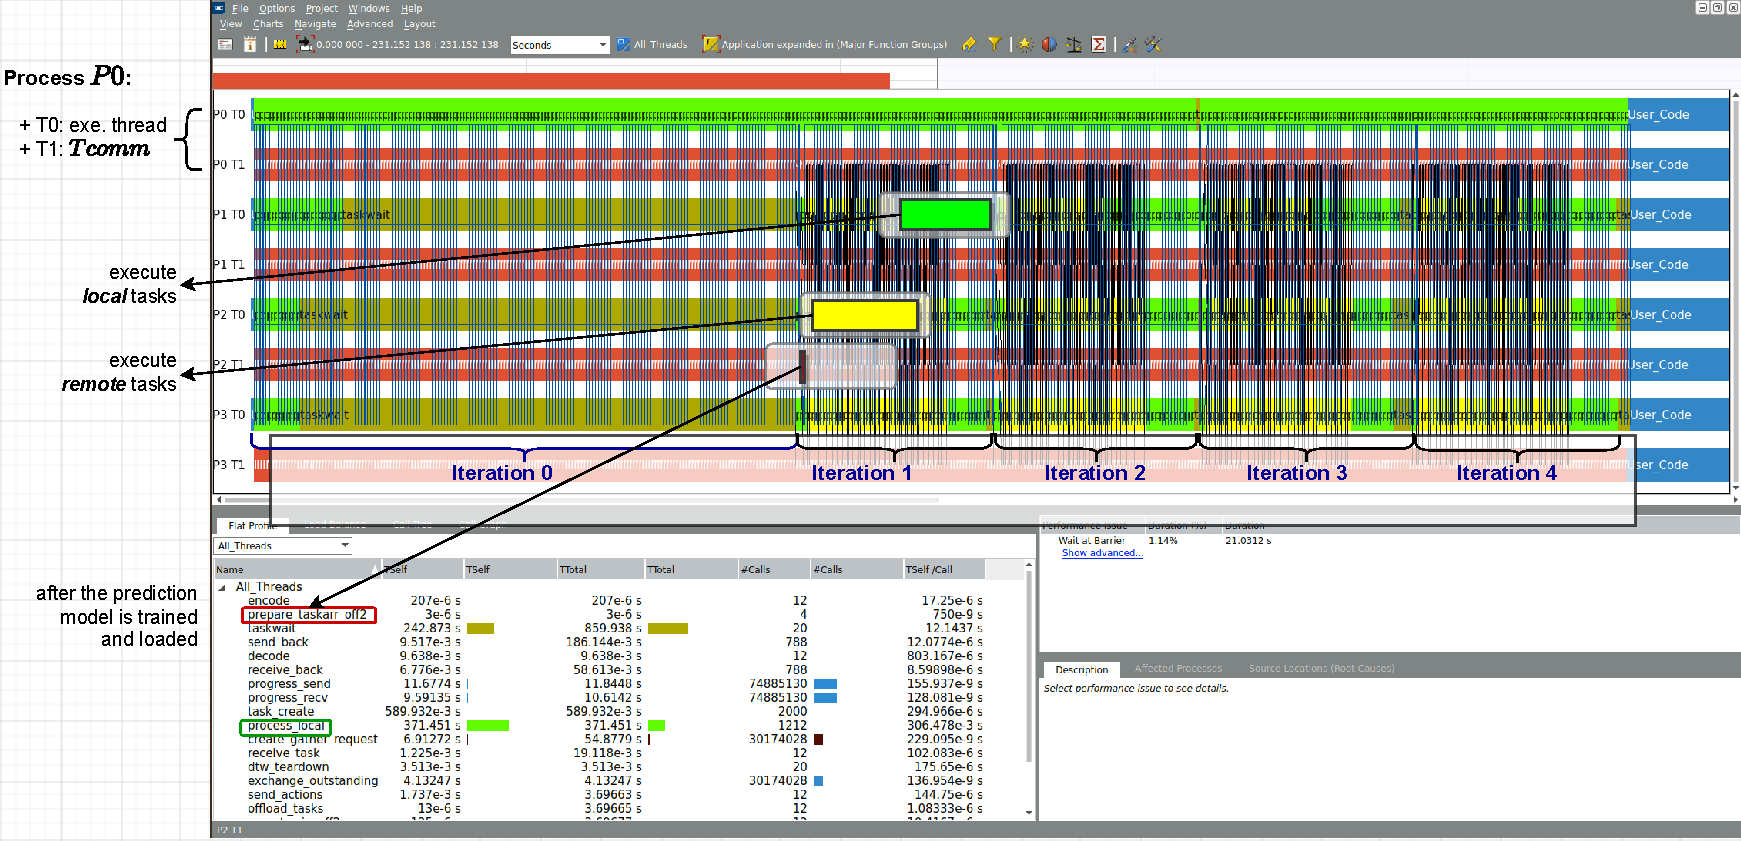
\includegraphics[scale=0.5125]{./pictures/poc_implementation/poc_visualize_trace_proactlb_off2.pdf}
	\caption{A visualization of Chameleon and the callback tool based on Intel Trace Analyzer and Collector.}
	\label{fig:poc_visualize_chamtool_trace_itac}
\end{figure}

Figure \ref{fig:poc_visualize_chamtool_trace_itac} shows a visualization of running Chameleon and our callback tool through most of the main operations profiled during execution. The visualization is conducted by Intel Trace Analyze and Collector (ITAC) \cite{wrinn2004mpiitac}. Due to the trace's scale and its overhead, this experiment is only a small test with $4$ MPI processes. The area with colors shows execution progress following the horizontal axis. On the left side, we can see processes labeled by $P0$, $...$, $P3$, the notations of task execution through colors, and the profiled information in the box at the bottom left corner. The experiment is shown over $5$ iterations, denoted by Iteration $0$, ... , Iteration $4$.\\

Each process has two threads denoted by $T0$ and $T1$, where one execution thread is created by OpenMP and one dedicated thread by POSIX thread. For example, Process $P0$ has $T0$ and $T1$, where $T0$ is the execution thread and $T1$ is $Tcomm$, as shown In Figure \ref{fig:poc_visualize_chamtool_trace_itac}. The green region indicates local tasks during execution, while the yellow one indicates remote tasks that are offloaded and executed on the remote side. In the first iteration, we can see that $P0$ is the bottleneck process with the most overloaded value without load balancing. During this iteration, $Tcomm$ on each process characterizes task features and records the load value per task. At the beginning of Iteration $1$, we mark a traced event called ``\texttt{prepare\_taskarr\_off2}'' to denote that the dataset is ready for training a prediction model after Iteration $0$. This callback event highlights the loaded prediction model for the upcoming iterations. Following that, in Iteration $1$, $2$, $3$, $4$, remote tasks are visualized with the execution on underloaded processes, and the imbalance is seen as significantly reduced.